\documentclass[14pt]{extarticle}
\usepackage[utf8]{inputenc}
\usepackage{tikz}
\usepackage{tkz-euclide}
\usetikzlibrary{calc,intersections,through,backgrounds}
%\usepackage{tikz} 
\usepackage{pdflscape}
\usepackage[margin=2cm]{geometry}
\usepackage{amsmath}
\usepackage{pgfplots}
\usepackage{cancel}
\usepackage{setspace}
\usepackage{fourier}

\setlength\parindent{0pt}
\pgfplotsset{compat=1.16}  
\usetikzlibrary{arrows.meta}

\begin{document}
\begin{center}
    \LARGE{\textbf{La Circonferenza e il Cerchio}}
\end{center}
\vspace{1cm}
\fbox{\begin{minipage}{1\textwidth}\textbf{Circonferenza:} La \textbf{circonferenza} è l'insieme di tutti i punti di un piano equidistanti da un punto fisse detto \textbf{centro}.
\end{minipage}}\vspace{0.5cm}
\fbox{\begin{minipage}{1\textwidth}\textbf{Cerchio:} Il \textbf{cerchio} è la parte di piano costituita dalla circonferenza e dai punti ad esse interni.
\end{minipage}}\vspace{1cm}


\begin{minipage}[t]{0.5\textwidth}
\begin{center}
\begin{tikzpicture}[scale=1]
    \tkzDefPoint(0,0){O}
    \tkzDefPoint(1.5,1.5){A}
    \tkzCalcLength(A,O) \tkzGetLength{rAO}
    \tkzDefCircle[R](O,\rAO) \tkzGetPoint{B}
    \tkzDrawCircle[color=red](O,B)
    %\tkzDrawSegment(O,A)
    %\tkzLabelSegment[above left](C,A){$2\sqrt{2}$}
    \tkzDrawPoints(O)
    \tkzLabelPoints(O)
\end{tikzpicture}\\
\textcolor{red}{Circonferenza}
\end{center}
\end{minipage}
\begin{minipage}[t]{0.5\textwidth}
\begin{center}

\begin{tikzpicture}[scale=1]
    \tkzDefPoint(0,0){O}
    \tkzDefPoint(3,3){B}
    \tkzDefCircle[diameter](O,B) \tkzGetPoint{A}
    \tkzDrawCircle[color=blue,fill=blue](A,B)
    %\tkzDrawPoints(A,B)
    %\tkzDrawSegment(A,B)
    %\tkzLabelPoints(O,A,B)
\end{tikzpicture}\\
\textcolor{blue}{Cerchio}
\end{center}
\end{minipage}\vspace{0.5cm}\\

\textbf{Parti di una circonferenza:}\\
\begin{itemize}
    \item \textbf{Raggio:} segmento che unisce il centro del cerchio e un qualsiasi punto sulla circonferenza. I raggi di una circonferenza sono \textbf{infiniti}.
        \begin{center}
            \begin{tikzpicture}[scale=1]
            \tkzDefPoint(0,0){O}
            \tkzDefPoint(1.5,1.5){A}
            \tkzCalcLength(A,O) \tkzGetLength{rAO}
            \tkzDefCircle[R](O,\rAO) \tkzGetPoint{B}
            \tkzDrawCircle(O,B)
            \tkzDrawSegment[color=blue](O,A)
            \tkzLabelSegment[above left](O,A){\(r\)}
            \tkzDrawPoints(O,A)
            \tkzLabelPoints(O)
            \tkzLabelPoints[above right](A)
            \end{tikzpicture}\\
        \textcolor{blue}{raggio \(r\)}
        \end{center}
    \item \textbf{Arco di circonferenza:} presi due punti A e B su una circonferenza, si chiama arco ciascuna delle due parti in cui la circonferenza viene divisa, si scrive con il simbolo\(\widearc{AB}\).\\
        \begin{center}
            \begin{tikzpicture}[scale=1]
            \tkzDefPoint(0,0){O}
            \tkzDefPoint(1.5,1.5){A}
            \tkzCalcLength(A,O) \tkzGetLength{rAO}
            \tkzDefCircle[R](O,\rAO) \tkzGetPoint{B}
            \tkzDrawCircle(O,B)
            %\tkzDrawSegment[color=blue](O,A)
            %\tkzLabelSegment[above left](O,A){\(r\)}
            \tkzDrawArc[color=red](O,B)(A)
            \tkzDrawArc[color=blue](O,A)(B)
            \tkzDrawPoints(O,A,B)
            \tkzLabelPoints(O)
            \tkzLabelPoints[above right](A)
            \tkzLabelPoints[right](B)
            \end{tikzpicture}\\
        \textcolor{red}{arco di circonferenza \(\widearc{AB}\) minore} e \textcolor{blue}{arco di circonferenza \(\widearc{AB}\) maggiore}
        \end{center}
    \item \textbf{Corda:} la corda di una circonferenza è ogni segmento che abbia gli estremi appartenenti alla circonferenza\\
        \begin{center} %\tkzDrawArc
            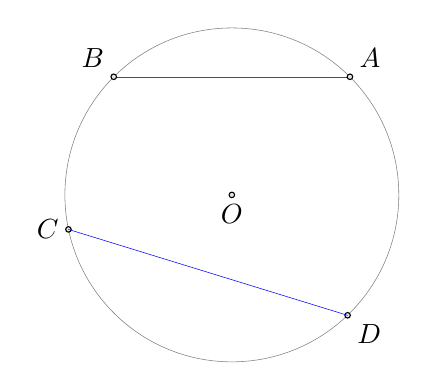
\begin{tikzpicture}[scale=1]
                \tkzDefPoint(0,0){O}
                \tkzDefPoint(1.5,1.5){A}
                \tkzDefPoint(-1.5,1.5){B}
                \tkzCalcLength(A,O) \tkzGetLength{rAO}
                \tkzDefCircle[R](O,\rAO)
                \tkzDrawCircle(O,A)
                \tkzDrawSegment[color=red](B,A)
                %\tkzLabelSegment[above left](C,A){$2\sqrt{2}$}
                \tkzDrawPoints(O,A,B)
                \tkzLabelPoints(O)
                \tkzLabelPoints[above right](A)
                \tkzLabelPoints[above left](B)
                \tkzDefPoint(3,-2){Lc}
                \tkzDefPoint(-10,2){Ld}
                %\tkzDrawSegment[color=red](Lc,Ld)
                \tkzInterLC(Lc,Ld)(O,A) \tkzGetPoints{C}{D}
                \tkzDrawPoints(C,D)
                \tkzLabelPoints[below right](D)
                \tkzLabelPoints[left](C)
                \tkzDrawSegment[color=blue](C,D)
            \end{tikzpicture}\\
        \textcolor{red}{corda \(\overline{AB}\)} e \textcolor{blue}{corda \(\overline{CD}\)}
        \end{center} 
    \item \textbf{Diametro:} il diametro di una circonferenza è ogni corda passante per il centro della circonferenza. Il diametro è sempre il doppio del raggio (\(d=2r\)) e ce ne sono infiniti.
    \begin{center} %\tkzDrawArc
            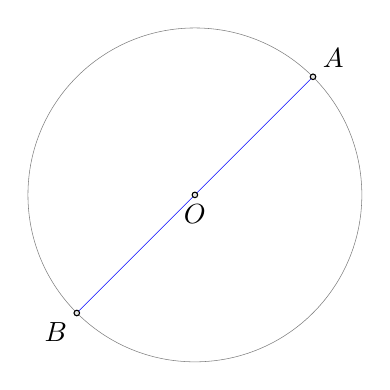
\begin{tikzpicture}[scale=1]
                \tkzDefPoint(0,0){O}
                \tkzDefPoint(1.5,1.5){A}
                \tkzDefPoint(-1.5,-1.5){B}
                \tkzCalcLength(A,O) \tkzGetLength{rAO}
                \tkzDefCircle[R](O,\rAO)
                \tkzDrawCircle(O,A)
                \tkzDrawSegment[color=blue](B,A)
                %\tkzLabelSegment[above left](C,A){$2\sqrt{2}$}
                \tkzDrawPoints(O,A,B)
                \tkzLabelPoints(O)
                \tkzLabelPoints[above right](A)
                \tkzLabelPoints[below left](B)
            \end{tikzpicture}\\
        \textcolor{blue}{diametro}
    \end{center} 
    \item \textbf{Semicirconferenza e semicerchio:} un diametro divide la circonferenza in due archi uguali, chiamati semicirconferenze e il cerchio in due parti di piano uguali, chiamate semicerchi.\\
    
    \begin{minipage}[t]{0.5\textwidth}
        \begin{center} %\tkzDrawArc
            \begin{tikzpicture}[scale=1]
                \tkzDefPoint(0,0){O}
                \tkzDefPoint(1.5,1.5){A}
                \tkzDefPoint(-1.5,1.5){B}
                \tkzCalcLength(A,O) \tkzGetLength{rAO}
                \tkzDefCircle[R](O,\rAO)
                \tkzDrawCircle(O,A)
                %\tkzLabelSegment[above left](C,A){$2\sqrt{2}$}
                \tkzDrawPoints(O)
                \tkzLabelPoints(O)
                \tkzDefPoint(4,0){Lc}
                \tkzDefPoint(-4,0){Ld}
                %\tkzDrawSegment[color=red](Lc,Ld)
                \tkzInterLC(Lc,Ld)(O,A) \tkzGetPoints{A}{B}
                \tkzDrawPoints(A,B)
                \tkzLabelPoints[right](A)
                \tkzLabelPoints[left](B)
                %\tkzDrawSegment[color=blue](A,B)
                \tkzDrawArc[color=red](O,B)(A)
                \tkzDrawArc[color=blue](O,A)(B)
            \end{tikzpicture}\\
        \textcolor{red}{Semicirconferenza \(\overline{AB}\)} e \textcolor{blue}{semicirconferenza \(\overline{CD}\)}
        \end{center} 
    \end{minipage}
    \begin{minipage}[t]{0.5\textwidth}
        \begin{center} %\tkzDrawArc
            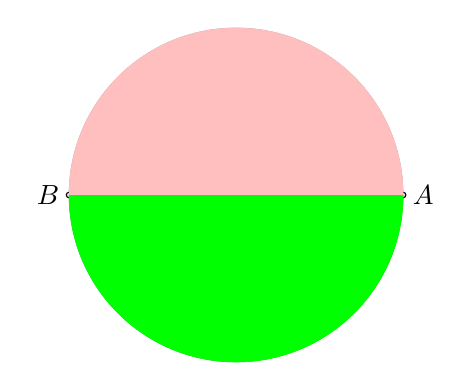
\begin{tikzpicture}[scale=1]
                \tkzDefPoint(0,0){O}
                \tkzDefPoint(1.5,1.5){A}
                \tkzDefPoint(-1.5,1.5){B}
                \tkzCalcLength(A,O) \tkzGetLength{rAO}
                \tkzDefCircle[R](O,\rAO)
                \tkzDrawCircle(O,A)
                %\tkzLabelSegment[above left](C,A){$2\sqrt{2}$}
                \tkzDrawPoints(O)
                \tkzLabelPoints(O)
                \tkzDefPoint(4,0){Lc}
                \tkzDefPoint(-4,0){Ld}
                %\tkzDrawSegment[color=red](Lc,Ld)
                \tkzInterLC(Lc,Ld)(O,A) \tkzGetPoints{A}{B}
                \tkzDrawPoints(A,B)
                \tkzLabelPoints[right](A)
                \tkzLabelPoints[left](B)
                %\tkzDrawSegment[color=blue](A,B)
                \tkzDrawSemiCircles[color=green, fill=green](O,B)
                \tkzDrawSemiCircles[color=pink, fill=pink](O,A)
            \end{tikzpicture}\\
        \textcolor{pink}{Semicerchio} e \textcolor{green}{semicerchio}
        \end{center} 
    \end{minipage}\\

Guardiamo adesso alcune \textbf{proprietà} di archi e corde.\\

\textbf{Proprietà 1:} La perpendicolare condotta dal centro di una circonferenza ad una corda divide tale corda a metà.\\


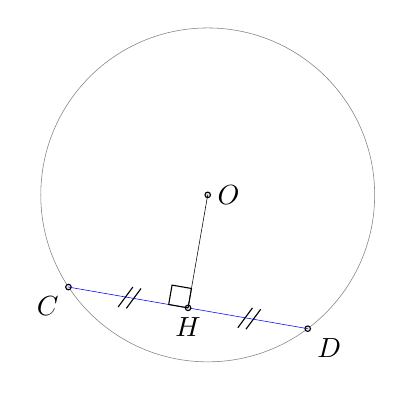
\begin{tikzpicture}[scale=1]
    \tkzDefPoint(0,0){O}
    \tkzDefPoint(1.5,1.5){A}
    \tkzDefPoint(-1.5,1.5){B}
    \tkzCalcLength(A,O) \tkzGetLength{rAO}
    \tkzDefCircle[R](O,\rAO)
    \tkzDrawCircle(O,A)
    %\tkzLabelSegment[above left](C,A){$2\sqrt{2}$}
    \tkzDrawPoints(O)
    \tkzLabelPoints[right](O)
    \tkzDefPoint(3,-2){Lc}
    \tkzDefPoint(-20,2){Ld}
    %\tkzDrawSegment[color=red](Lc,Ld)
    \tkzInterLC(Lc,Ld)(O,A) \tkzGetPoints{C}{D}
    \tkzDrawPoints(C,D)
    \tkzLabelPoints[below left](C)
    \tkzLabelPoints[below right](D)
    \tkzDrawSegment[color=blue](C,D)
    \tkzDefPointBy[projection=onto C--D](O) \tkzGetPoint{H}
    \tkzDrawSegment[](O,H)
    \tkzDrawPoints(H)
    \tkzLabelPoints(H)
    \tkzMarkRightAngle(C,H,O)
    \tkzMarkSegments[mark=s||](C,H H,D)
\end{tikzpicture}\\

\textbf{Proprietà 2:} in una stessa circonferenza ad archi congruenti corrispondono corde congruenti e viceversa.\\

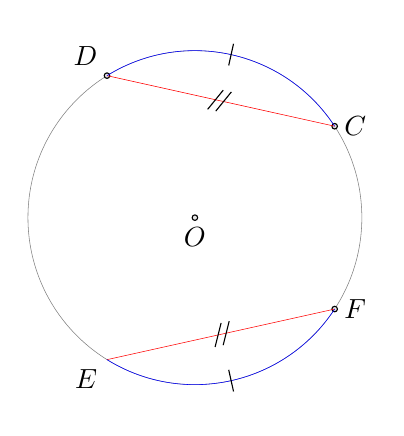
\begin{tikzpicture}[scale=1]
    \tkzDefPoint(0,0){O}
    \tkzDefPoint(1.5,1.5){A}
    %\tkzDefPoint(-1.5,1.5){B}
    \tkzDefPoint(7,0){Lc}
    \tkzDefPoint(-2,2){Ld}
    \tkzDefPoint(-2,-2){Le}
    \tkzCalcLength(A,O) \tkzGetLength{rAO}
    \tkzDefCircle[R](O,\rAO)
    \tkzDrawCircle(O,A)
    %\tkzDrawSegment[color=red](B,A)
    %\tkzLabelSegment[above left](C,A){$2\sqrt{2}$}
    \tkzDrawPoints(O)
    \tkzLabelPoints(O)
    %\tkzDrawSegment[color=red](Lc,Ld)
    \tkzInterLC(Lc,Ld)(O,A) \tkzGetPoints{C}{D}
    \tkzInterLC(Lc,Le)(O,A) \tkzGetPoints{E}{F}
    \tkzDrawPoints(C,D,F)
    \tkzLabelPoints[right](C,F)
    \tkzLabelPoints[above left](D)
    \tkzLabelPoints[below left](E)
    \tkzDrawSegment[color=red](C,D)
    \tkzDrawSegment[color=red](E,F)
    \tkzMarkSegments[mark=s||](C,D E,F)
    \tkzDrawArc[color=blue](O,C)(D)
    \tkzDrawArc[color=blue](O,E)(F)
    \tkzMarkArc[mark=|](O,C,D)
    \tkzMarkArc[mark=|](O,E,F)
\end{tikzpicture}\\
\clearpage
Viste queste proprietà passiamo ad un \\
\textbf{Teorema:} \textit{due corde congruenti (stessa lunghezza) di una stessa circonferenza hanno la stessa distanza dal centro.}\\

\begin{minipage}[c]{0.3\textwidth}
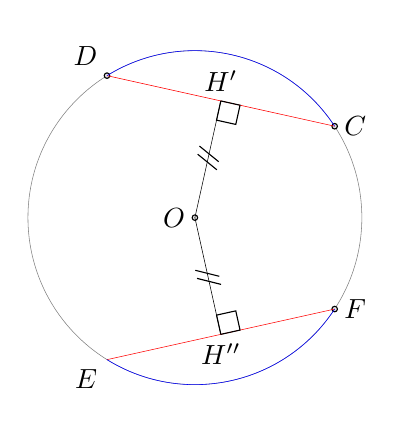
\begin{tikzpicture}[scale=1]
    \tkzDefPoint(0,0){O}
    \tkzDefPoint(1.5,1.5){A}
    %\tkzDefPoint(-1.5,1.5){B}
    \tkzDefPoint(7,0){Lc}
    \tkzDefPoint(-2,2){Ld}
    \tkzDefPoint(-2,-2){Le}
    \tkzCalcLength(A,O) \tkzGetLength{rAO}
    \tkzDefCircle[R](O,\rAO)
    \tkzDrawCircle(O,A)
    %\tkzDrawSegment[color=red](B,A)
    %\tkzLabelSegment[above left](C,A){$2\sqrt{2}$}
    \tkzDrawPoints(O)
    \tkzLabelPoints[left](O)
    %\tkzDrawSegment[color=red](Lc,Ld)
    \tkzInterLC(Lc,Ld)(O,A) \tkzGetPoints{C}{D}
    \tkzInterLC(Lc,Le)(O,A) \tkzGetPoints{E}{F}
    \tkzDrawPoints(C,D,F)
    \tkzLabelPoints[right](C,F)
    \tkzLabelPoints[above left](D)
    \tkzLabelPoints[below left](E)
    \tkzDrawSegment[color=red](C,D)
    \tkzDrawSegment[color=red](E,F)
    \tkzDrawArc[color=blue](O,C)(D)
    \tkzDrawArc[color=blue](O,E)(F)
    \tkzDefPointBy[projection=onto C--D](O) \tkzGetPoint{H'}
    \tkzDrawSegment[](O,H')
    \tkzDefPointBy[projection=onto E--F](O) \tkzGetPoint{H''}
    \tkzDrawSegment[](O,H'')
    \tkzLabelPoints[above](H')
    \tkzLabelPoints[below](H'')
    \tkzMarkSegments[mark=s||](O,H' O,H'')
    \tkzMarkRightAngle(C,H',O)
    \tkzMarkRightAngle(F,H'',O) 
\end{tikzpicture}
\end{minipage}
\begin{minipage}[c]{0.7\textwidth}
\(\overline{EF}\cong\overline{CD}\)\\     
\(\overline{OH'}\cong\overline{OH''}\)
\end{minipage}\\

\small{\textit{[Come puoi dimostrare questo teorema? Mica vorrai saperlo ricordandotelo solo a memoria vero?]}}\\
\clearpage
\begin{center}
    \large{\textbf{Posizioni di una retta rispetto ad una circonferenza}}\\
\end{center}
In un piano possiamo identificare 3 casi di posizioni di una retta rispetto ad una circonferenza.\\

\textbf{Caso 1)} La retta e la circonferenza non hanno alcun punto in comune.\\

\textbf{Caso 2)} La retta e la circonferenza hanno due punti in comune.\\

\textbf{Caso 3)} La retta e la circonferenza hanno un solo pnto in comune.\\


\end{itemize}


\end{document}


